\documentclass[11pt]{article}
    \usepackage{comment} % enables the use of multi-line comments (\ifx \fi) 
    \usepackage{lipsum} %This package just generates Lorem Ipsum filler text. 
    \usepackage{fullpage} % changes the margin
    % Used for importing figures
    \usepackage{graphicx}
    \usepackage{wrapfig}
    \usepackage{float}
    \usepackage{subcaption}
    
\begin{document}

%Header-Make sure you update this information!!!!
\noindent
\large\textbf{Lab 6} \hfill \textbf{Zach Colbert} \\
\normalsize PH 411 \hfill 28 November 2017\\

\section*{Introduction}
In the second lab on op-amps, we take a look at some new features since the last lab--some of which can be very useful for building new circuits, some of which have drawbacks or impose limits on normal operation of op-amps. We also take a look at the ways that positive feedback changes the behavior of a circuit, in comparison to the negative feedback we used in Lab 6.\\


\section{Slew Rate}
\subsection{Experimental}

Op-amps have a property called the \emph{slew rate}, which defines how fast an amplifier can react to sudden changes in their input signal. This is significant because it essentially places a limit on how fast our input signal can cycle before the output signal looks significantly different than we expect.\\

By building a simple circuit around an op-amp, we're able to see this distortion very clearly. We're also able to measure the slew rate of the op-amp by inputting a square wave (the most abrupt signal changes we could possibly make) and measuring the change of the output signal with respect to time in regions where the input signal changes. This measurement of the slope of our output signal, and the literature value for the slew rate, come in units of $V / \mu s$.\\

\begin{figure}[H]
    \centering
    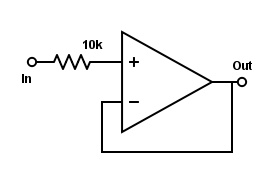
\includegraphics[scale=0.5]{Diagrams/c-a.png}
    \caption{A simple op-amp circuit with negative feedback. The output of this signal demonstrates the distortion caused by the slew rate of the amplifier.}
    \label{circuit:a}
\end{figure}


\subsection{Results}

Using an LM-741 op-amp, and applying a $3\ V$ peak-to-peak square wave at $10\ kHz$, we recorded the output signal shown in figure \ref{fig:A-1}.\\

\begin{figure}[H]
    \centering
    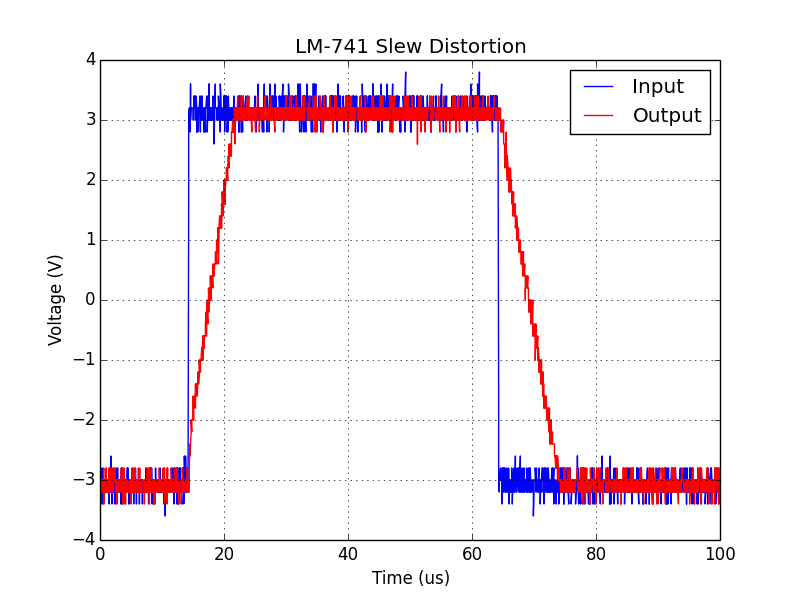
\includegraphics[scale=0.6]{Plots/figA-1.png}
    \caption{Slew distortion of circuit \ref{circuit:a}, using an LM-741 amplifier.}
    \label{fig:A-1}
\end{figure}

We find that the slew rate on the rising edge is about $0.8\ V / \mu s$, and on the falling side is about $0.6 V / \mu s$. Both values are reasonably close to the literature value \footnote{Found in the datasheet at http://www.ti.com/lit/ds/symlink/lm741.pdf} $0.5\ V / \mu s$.\\

For the same device, we also applied a sine wave input for comparison. At $10\ kHz$ we were unable to see any distortion for any input voltage--however, we began to see distortion at $3\ V_{pp}$ near $50\ kHz$. It seems reasonable that we had to increase input frequency by a factor in order to see distortion effects on a sine wave, considering the rate of change of a sine wave is much lower than that of a square wave.\\ 

\begin{figure}[H]
    \centering
    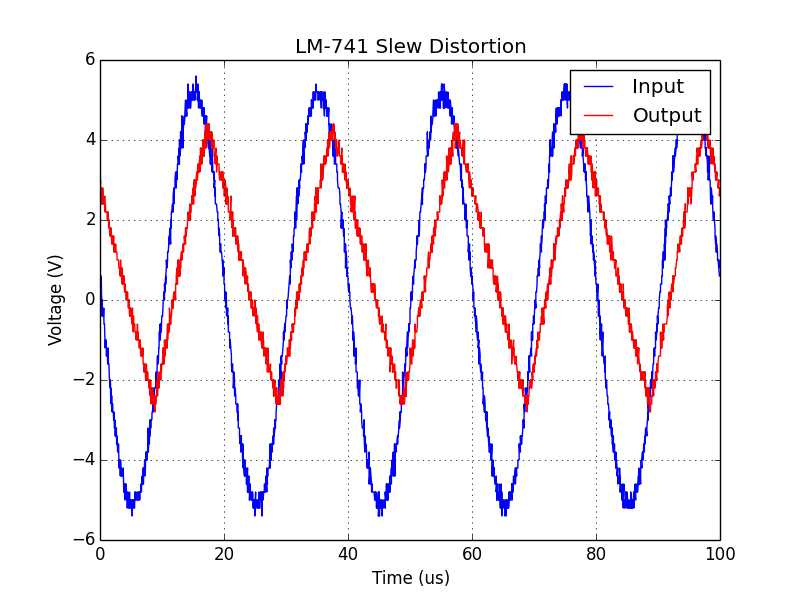
\includegraphics[scale=0.6]{Plots/figA-2.png}
    \caption{Slew distortion of circuit \ref{circuit:a}, using an LM-741 amplifier.}
    \label{fig:A-2}
\end{figure}

For the rising and falling edges of this output signal, we found the slew rate to be about $0.6\ V / \mu s$, closer to the literature value.\\

Using a TL-071 amplifier in the same circuit, we applied the same square wave input as above and found the slew rate to be $12\ V / \mu s$, compared to the $13\ V / \mu s$ literature value \footnote{Found in the datasheet at http://www.ti.com/lit/ds/symlink/tl072a.pdf}. For this amplifier, we had to increase the input frequency to around $900\ kHz$ before we saw similar distortion on a sine wave--and found the slew rate there to be about $8\ V / \mu s$, which is given as the minimum slew rate in literature.

Because the rate of change of a sine wave is smaller than that of a square wave, it made sense for us to have increased the input frequency by a small factor for the first amplifier. Changing the frequency by an order of magnitude for the second amplifier isn't quite as reasonable--there is probably some other factor that is affecting the frequency-dependence of the slew rate, but I haven't been able to identify it.


\section{Offset Voltage}
\subsection{Results}

One of the features of op-amps is the \emph{offset voltage}. This DC voltage determines the default offset between the two input voltages, and can be adjusted by applying a DC signal to two of the pins on the amplifier. 

\begin{figure}[H]
    \centering
    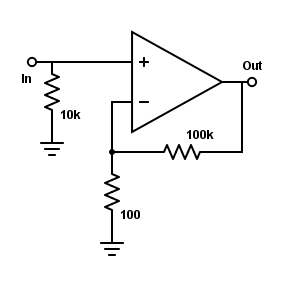
\includegraphics[scale=0.5]{Diagrams/c-b1.png}
    \caption{This non-inverting amplifier circuit has a gain of 1000. With the input grounded, we can measure the DC offset voltage of the op-amp.}
    \label{circuit:b1}
\end{figure}

Circuit \ref{circuit:b1}, with the input grounded, can be used to measure the offset voltage of the amplifier. Because there is zero voltage at the non-inverting input, and some offset voltage between that and the inverting input, the circuit will output the offset voltage multiplied by the circuit gain.

\begin{figure}[H]
    \centering
    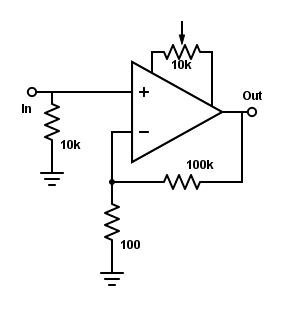
\includegraphics[scale=0.5]{Diagrams/c-b2.png}
    \caption{The addition to the circuit at pins 1 and 5 on the op-amp is very simple, and allows us to adjust the DC offset voltage easily.}
    \label{circuit:b2}
\end{figure}

By adding applying a DC signal to pins 1 and 5 of the op-amp through a potentiometer, we're able to adjust or "trim" the offset voltage. 


\subsection{Results}

With the input of the circuit grounded, we were able to measure a DC signal around $800\ mV$, which translates to an offset voltage of about $0.8\ mV$ considering the circuit gain of 1000. According to the datasheet for the LM-741 amplifier, the offset voltage is typically $1\ mV$. 

The $10\ k \Omega$ potentiometer was not too sensitive for trimming this circuit, and we were able to adjust it so that the circuit output was very near zero with the input grounded.


\section{Integrator}
\subsection{Experimental}

As we did in earlier labs with passive elements, op-amps can also be used to build circuits that integrate or differentiate their input signals. These circuits have a number of applications already, and the use of an active element gives us extra functionality.

\begin{figure}[H]
    \centering
    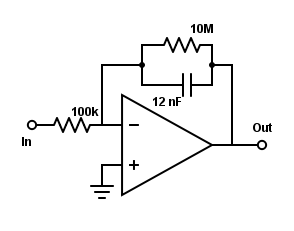
\includegraphics[scale=0.5]{Diagrams/c-c.png}
    \caption{An integrator circuit that employs active and passive elements, including an op-amp.}
    \label{circuit:c}
\end{figure}

In this part of the lab, we observe the resulting signal of different kinds of input, and use those to analyze the circuit's behavior as an integrator.


\subsection{Results}

Driving the circuit with a $1\ V$ peak-to-peak square wave at $1\ kHz$ resulted in a triangle wave output, with a much smaller amplitude (suggesting gain $\beta < 1$) and a significant DC offset\footnote{Note: We removed the offset trimming circuitry from the previous circuit while building the circuit for this part of the lab, so the offset voltage of the amplifier could have played some part in the DC offset of this signal.}. The type of output signal matches what we would expect from an integrator--regions of a triangle wave have constant rate of change, represented by the constant values of a square wave.

This integrating behavior was consistent for similar sine and triangle inputs as well.

Adjusting the DC offset of the input signal (via our function generator) also changed the DC offset of the output signal, with a noticeable ($>1$) gain, opposite the direction of the input offset change (positive offset of the input signal resulted in negative offset of the output signal). 


\end{document}
